% Baccalauréat malgache, série C, 2011 : énoncé.
\TCDBacAttribution{C}{2011}
\providecommand{\dx}{\mathrm{d}x}
\providecommand{\Re}[1]{\mathrm{Re}\left( #1 \right)}
\providecommand{\Im}[1]{\mathrm{Im}\left( #1 \right)}
\providecommand{\dt}{\mathrm{d}t}
\providecommand{\Ouv}{(O;\vec{u},\vec{v})}
\providecommand{\mes}[2]{\mathrm{mes}\left( \widehat{ \overrightarrow{#1} ; \overrightarrow{#2} } \right)}
\providecommand{\D}{(\mathscr{D})}
\providecommand{\Courbe}{(\mathscr{C})}
\providecommand{\congru}[3]{#1 \equi #2 \quad \left[ \mathrm{mod}~#3\right]}
%
%%%%%%%%%%%%%%%%%%%%%%%%%%%%%%%%%%%%%%%%%%%%%%%%%%%%%%%%%%%%%%%%%%%%%%%%%%%%%%%%%%%%%%%%%%%%%%%%%%%%%%%%%%%%%%%%%%%%%%%%%%%%%%%%
\noindent \underline{\textsc{\textbf{Exercice}}} (4 points) \\%[-1\baselineskip]
      \underline{A- Probabilit\'e.} \newline
      On dispose d'un d\'e cubique parfait dont les faces sont num\'erot\'ees : 0, 1, 1, 2, 2 et 2.
      \begin{enumerate}
            \item On lance une fois ce d\'e. 
                  Calculer les probabilit\'es $P_0$, $P_1$, $P_2$ d'apparition respectives des faces num\'erot\'ees 0, 1, 2.
            \item Une \'epreuve consiste \`a lancer trois fois de suite ce d\'e et d'une mani\`ere ind\'ependante.
                  On note chaque fois le num\'ero obtenu sur la face sup\'erieure de ce d\'e.
                  Calculer la probabilit\'e de chacun des \'ev\`enements suivants :
                  \begin{description}
                        \item[$A$ :] << La somme des num\'eros obtenus est \'egale \`a 4 >>.
                        \item[$B$ :] << Obtenir exactement deux fois le num\'ero 1 >>.
                        \item[$C$ :] << Obtenir chacun des trois num\'eros diff\'erents lors des 3 lancers >>.
                  \end{description}
      \end{enumerate}

            \hspace{\stretch{1}}
            \textbf{\underline{NB :} On donnera les r\'esultats sous forme de fraction irr\'eductible.}
            \hspace{\stretch{1}}

      \underline{B- Arithm\'etique.} 
      \begin{enumerate}
            \item \begin{enumerate}
                        \item Convertir dans la base 10 l'entier $a$ \'ecrit dans le syst\`eme binaire : 
                              $a = \overline{(1011101)_2}$.
                        \item Convertir dans le syst\`eme binaire l'entier naturel $b = 54$ de la base 10.
                  \end{enumerate}
            \item \begin{enumerate}
                        \item Dresser la table d'addition et de multiplication de $\mathbb{Z}/5\mathbb{Z}$.
                        \item R\'esoudre dans $\mathbb{Z}/5\mathbb{Z} \times \mathbb{Z}/5\mathbb{Z}$ le syst\`eme : 
                              $
                                    \begin{multiform}
                                          \bar{3} x + \bar{2} y = \bar{1} \\
                                          \bar{2} x + \bar{4} y = \bar{3} \;.
                                    \end{multiform}
                              $ 
                        \item R\'esoudre l'\'equation : $x^2 - x - \bar{2} = \bar{0}$ dans $\mathbb{Z}/5\mathbb{Z}$.
                  \end{enumerate}
      \end{enumerate}
%%%%%%%%%%%%%%%%%%%%%%%%%%%%%%%%%%%%%%%%%%%%%%%%%%%%%%%%%%%%%%%%%%%%%%%%%%%%%%%%%%%%%%%%%%%%%%%%%%%%%%%%%%%%%%%%%%%%%%%%%%%%%%%%
\noindent \underline{\textsc{\textbf{PROBLEME I}}} (7 points) \newline
%      \begin{minipage}[t]{1\actualtextwidth-5.5cm}
            $ABEC$ est un losange de centre $O$ dans un plan orient\'e $\Plan$ tel que : 
            $AB = AC = BC = 4\cm$ et $\Angl{AB}{AC} = \frac{\pi}{3}$.
            
            \hspace{\stretch{1}}
            \textbf{Les parties A et B sont ind\'ependantes.}
            \hspace{\stretch{1}}
            
%      \end{minipage}
      %
%      \begin{minipage}[t]{5cm} ~\newline
      \begin{figure}[h!]
      \centering
            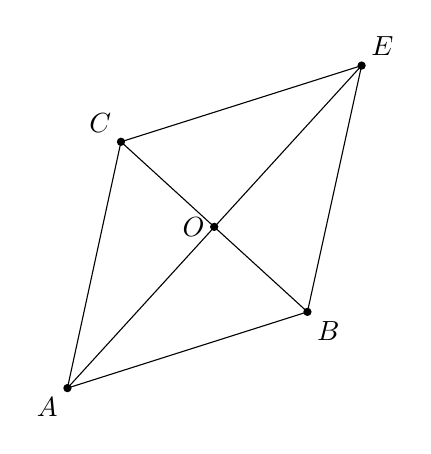
\begin{tikzpicture}[x=.8cm,y=.8cm]
                  %\clip(0.5,-1.5) rectangle (7,4.75);
                  \draw (1.52,-0.88)-- (5.33,0.33);
                  \draw (5.33,0.33)-- (6.19,4.24);
                  \draw (6.19,4.24)-- (2.37,3.03);
                  \draw (2.37,3.03)-- (1.52,-0.88);
                  \draw (1.52,-0.88)-- (6.19,4.24);
                  \draw (2.37,3.03)-- (5.33,0.33);
                  \fill [color=black] (1.52,-0.88) circle (1.5pt) node[below left] {$A$};
                  \fill [color=black] (5.33,0.33) circle (1.5pt) node[below right] {$B$};
                  \fill [color=black] (2.37,3.03) circle (1.5pt) node[above left] {$C$};
                  \fill [color=black] (6.19,4.24) circle (1.5pt) node[above right] {$E$};
                  \fill [color=black] (3.85,1.68) circle (1.5pt) node[left] {$O$};
            \end{tikzpicture}
      \end{figure}
%      \end{minipage}
      
      \textbf{\underline{Partie A}} 
      \begin{enumerate}
            \item Reproduire cette figure en vraie grandeur.
            \item \begin{enumerate}
                        \item On consid\`ere le syst\`eme de points pond\'er\'es 
                              $J = \{ (A,2);(B,1);(C,1) \}$.
	                              Montrer que ce syst\`eme admet un barycentre $G$ et que $G$ est le milieu du segment $[OA]$.
                        \item Montrer que le vecteur $-2\overrightarrow{MA} + \overrightarrow{MB} + \overrightarrow{MC}$
                              o\`u $M$ est un point variable, est un vecteur constant que l'on d\'eterminera.
                        \item D\'eterminer et repr\'esenter l'ensemble $\D$ des points $M$ du plan $\Plan$ v\'erifiant
                              \[
                                \begin{aligned}
                                  &\left(2\overrightarrow{MA}+\overrightarrow{MB}+\overrightarrow{MC}\right)
                                  \mathbin{\cdot} \\
                                  &\qquad\left(-2\overrightarrow{MA}+\overrightarrow{MB}+\overrightarrow{MC}\right)=0.
                                \end{aligned}
                              \]
                  \end{enumerate}
            \item Soit $S$ la similitude plane directe de rapport $\frac{1}{2}$, 
                  d'angle $\frac{\pi}{3}$ et qui transforme $A$ en $B$.
                  On note $I$ le centre de $S$ et $I'$ son image par la sym\'etrie centrale $S_B$ de centre $B$.
                  \begin{enumerate}
                        \item Montrer que le triangle $IAI'$ est un triangle \'equilat\'eral de sens direct.
                        \item Montrer que $\Angl{AB}{AI} = \frac{\pi}{6}$.
                        \item Placer alors les points $I$ et $I'$.
                  \end{enumerate}
      \end{enumerate}
      %
      \underline{\textbf{Partie B} (Utilisation des nombres complexes.)} 
      On rapporte le plan $\Plan$ au rep\`ere orthonorm\'e direct 
      $(A;\vec{u},\vec{v})$ avec $\vec{u} = \frac{1}{4} \overrightarrow{AB}$ ($\|\vec{u}\| = \|\vec{v}\|$).
      \begin{enumerate}
            \item \begin{enumerate}
                        \item Donner les affixes $z_A$ et $z_B$ respectives de $A$ et $B$.
                        \item Donner le module et un argument de l'affixe $z_C$ de $C$ et en d\'eduire l'affixe $z_C$
                              sous forme alg\'ebrique.
                        \item Calculer l'affixe $z_O$ de $O$.
                  \end{enumerate}
            \item \begin{enumerate}
                        \item Donner l'expression complexe de la similitude directe 
                              $S$ de rapport $\frac{1}{2}$ et d'angle $\frac{\pi}{3}$, qui transforme $A$ en $B$.
                        \item En d\'eduire l'affixe $z_I$ du centre $I$ de $S$.
                        \item V\'erifier que $\frac{z_I}{z_O}$ est un nombre r\'eel et que 
                              $\frac{z_B - z_I}{z_B - z_A}$ est imaginaire pur.
                        \item Que peut-on en d\'eduire pour les points $I$, $O$ et $A$ d'une part
                              et pour les droites $(IB)$ et $(AB)$ d'autre part\,?
                  \end{enumerate}
      \end{enumerate}
%%%%%%%%%%%%%%%%%%%%%%%%%%%%%%%%%%%%%%%%%%%%%%%%%%%%%%%%%%%%%%%%%%%%%%%%%%%%%%%%%%%%%%%%%%%%%%%%%%%%%%%%%%%%%%%%%%%%%%%%%%%%%%%%
\noindent \underline{\textsc{\textbf{PROBLEME II}}} (9 points) \newline
      Soit $f$ la fonction num\'erique d\'efinie sur $\mathbb{R}$ par : $f(x) = \expo{\frac{x}{2}} - x - 1$.
      On d\'esigne par $\Courbe$ sa courbe repr\'esentative dans un rep\`ere orthonorm\'e \Oij{} d'unit\'e $2\cm$.
      \begin{description}
            \item[Partie A : ] Etude de la fonction $f$. \\[-1\baselineskip]
                  \begin{enumerate}
                        \item Calculer $\lim_{x\rightarrow -\infty} f(x)$ et $\lim_{x\rightarrow +\infty} f(x)$.
                              (Pour la limite en $+\infty$, poser $X = \frac{x}{2}$)
                        \item \begin{enumerate}
                                    \item Etudier les variations de $f$.
                                    \item Montrer que la droite $\D$ d'\'equation $y = - x - 1$ est asymptote \`a $\Courbe$.
                                    \item Montrer que l'\'equation $f(x) = 0$ admet pour solution $0$ et $\alpha$ dans 
                                          $\mathbb{R}$ et que $2 < \alpha < 3$.
                              \end{enumerate}
                        \item Tracer $\Courbe$ et $\D$ dans un m\^eme rep\`ere.
                              
                              \hspace{\stretch{1}}
                                    On donne $\expo{} = 2,7$ ; $\expo{\frac{3}{2}} = 4,48$ et pour la construction,
                                    on prendra $\alpha = 2,5$.
                              \hspace{\stretch{1}}
                        \item Soit $\lambda$ un nombre r\'eel strictement inf\'erieur \`a $-1$.
                              \begin{enumerate}
                                    \item Exprimer en fonction de $\lambda$ l'aire $A(\lambda)$, en $\cm^2$,
                                          de la portion du plan d\'elimit\'ee par la courbe $\Courbe$,
                                          la droite $\D$ et les droites d'\'equations respectives $x=\lambda$ et $x = -1$.
                                    \item Calculer $\lim_{\lambda\rightarrow -\infty} A(\lambda)$.
                              \end{enumerate}
                  \end{enumerate}
            \item[Partie B : ] Etude d'une suite. \newline
                  On consid\`ere la fonction num\'erique $g$ d\'efinie sur $]-1 ; +\infty[$ par $g(x) = 2 \ln (x+1)$.
                  \begin{enumerate}
                        \item Etudier les variations de la fonction $g$.
                        \item Montrer que $\alpha$ est solution de l'\'equation $g(x) = x$.
                        \item Montrer que pour tout $x \in [2 ; +\infty[$, $g(x) \in ]2 ; +\infty[$.
                        \item $(U_n)_{n\in\mathbb{N}}$ est la suite num\'erique d\'efinie par $U_0 = 3$
                              et $U_{n+1} = g(U_n)$ et que tous les termes de la suite appartiennent \`a $[2;+\infty[$
                              (on ne demande pas de le d\'emontrer).
                              \begin{enumerate}
                                    \item D\'emontrer que pour tout $x \in [ 2; +\infty[$, on a $|g'(x)| \leq \frac{2}{3}$.
                                    \item D\'emontrer, en utilisant le th\'eor\`eme des in\'egalit\'es des accroissements
                                          finis, que pour tout $n \in \mathbb{N}$, on a :
                                          $
                                                |U_{n+1} - \alpha | \leq \frac{2}{3} |U_n - \alpha |
                                          $ et que 
                                          $
                                                |U_n - \alpha| \leq \left( \frac{2}{3} \right)^n \;.
                                          $
                                    \item Prouver que la suite $(U_n)$ converge vers un r\'eel $\ell$ que l'on d\'eterminera.
                                    \item D\'eterminer l'entier naturel $p$ tel que, pour tout entier naturel $n$
                                          sup\'erieur ou \'egal \`a $p$, on ait :
                                          $| U_n - \alpha | \leq 10^{-4}$.
                              \end{enumerate}
                  \end{enumerate}
      \end{description}
%%%%%%%%%%%%%%%%%%%%%%%%%%%%%%%%%%%%%%%%%%%%%%%%%%%%%%%%%%%%%%%%%%%%%%%%%%%%%%%%%%%%%%%%%%%%%%%%%%%%%%%%%%%%%%%%%%%%%%%%%%%%%%%%

































